\subsubsection{Sedov Explosion}
\label{sec.tests.sedov}

\begin{figure}
\begin{center}
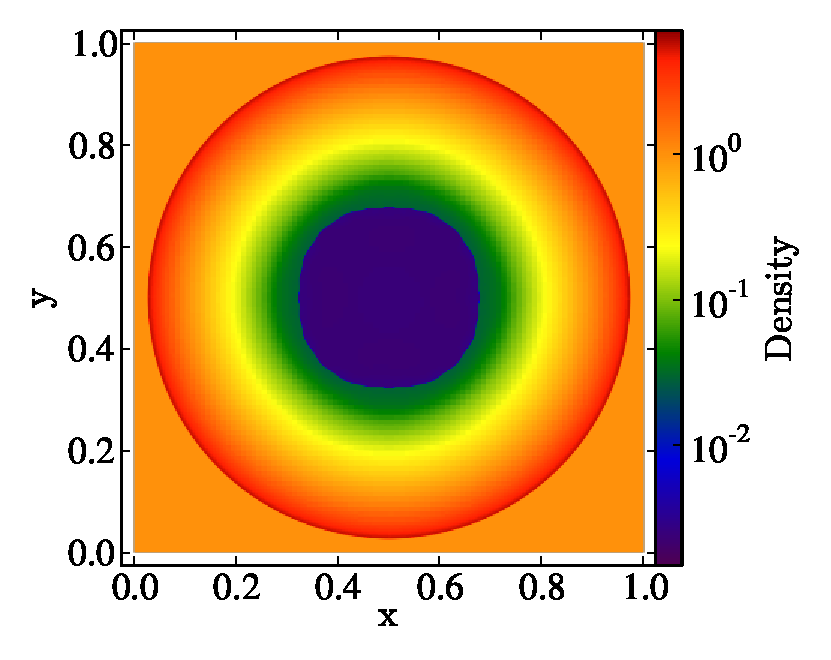
\includegraphics[width=0.4\textwidth]{figures/sedov-ppm-slice.eps}
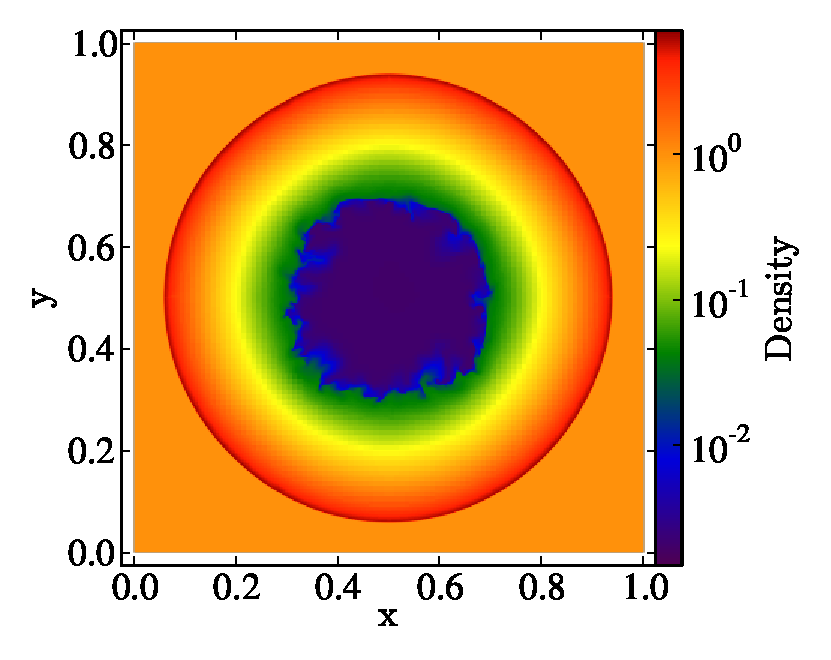
\includegraphics[width=0.4\textwidth]{figures/sedov-zeus-slice.eps}
\caption{Density slice from the Sedov Blast test at $t = 0.07$. Left:
results using the Piecewise Parabolic Method hydro scheme.  Right: results using the \zeus\
hydro method. Notably, the \zeus\ shock front has progressed less far
than in the PPM run. This is due to energy loss when conserving only
internal, and not total, energy.}
\label{fig.sedov1}
\end{center}
\end{figure}


\begin{figure}
\begin{center}
\includegraphics[width=\textwidth]{figures/sedov-profiles.eps}
\caption{Radially averaged profiles for the Sedov Blast test at $t =
0.07$. Clockwise from top-left shows density, velocity, internal
energy and pressure.  The black solid line shows the analytic
solution.  The blue dashed line shows the simulation using the PPM
method, and the red dot-dashed line using \zeus.  The \zeus\ result
substantially lags the true result due to total energy not being
explicitly converged.}
\label{fig.sedov2}
\end{center}
\end{figure}

The Sedov Blast Test \citep{Sedov1959} models an intense explosion,
initiated by depositing thermal energy into a homogenous distribution
of gas. The result is a strong spherical shock wave centered on the
point of energy injection.  This problem is a popular test of
astrophysical numerical codes for three reasons: First, it is
particularly appropriate to astrophysics since it represents the
situation when a supernovae explosion occurs. Second, it has an
exact analytical solution whereby the shock front's radial position is
given by:

\begin{equation} r(t) =
\left(\frac{E_0}{\alpha\rho_0}\right)^{1/5}t^{2/5}
\end{equation}

\noindent where $E_0$ is the initial energy injection, $\rho_0$ is the
background density and $\alpha = 1.0$ for cylindrical symmetry and an
ideal gas with $\gamma = 1.4$. For the full derivation see
\citet{Sedov1959}. This solution makes it possible to assess how well
the code performs.  Third, the spherical shock is a challenging
problem for numerical codes (both grid and particle) since the shock
wave increases in size as the simulation progresses and its
symmetrical nature highlights any directional preferences that grid
codes can succumb to. The test presented here is the two-dimensional
version that is included in the \enzo\ distribution. The
three-dimensional results from this test, both for \enzo\ and three
other leading astrophysics codes, can be founds in \citet{Tasker2008}.

In the initial state, the box contains a homogenous distribution of
gas at a density of 1 (note that, in the absense of gravity, this
problem is scale-free and thus without units). Thermal energy is
deposited into a single cell at the center of the box with $E_0 =
10.0$. The problem is completed in two dimensions with reflecting
boundary conditions (the default for \enzo) and uses a box size of side
$1$. For this problem, we selected a top grid of $100 \times 100$
cells and a maximum of four levels of refinement, placed based on
shock location and the slope in density and total energy. The
exception to this scheme is in the initial conditions, where grids are
placed directly around the injection point. The results were assessed
at $t = 0.07$, which corresponding to a time just before the shock
reaches the box edge (see Figure~\ref{fig.sedov1}).

Figure~\ref{fig.sedov2} shows the radial profiles for the simulation
run with the PPM hydro-solver (blue dashed line) and the \zeus\
hydro-solver (red dash-dot-dot line) together with the analytical
solution (black solid line). Clockwise from the top-left are density,
velocity, internal energy and pressure. PPM matches the analytical
solution extremely well for all quantities. However, the shock front
in the \zeus\ simulation lags behind the analytical position. This can
also be seen in the slices shown in Figure~\ref{fig.sedov1}. The cause
of this discrepancy is that \zeus\ shows a substantial energy loss
during the first few timesteps and produces a diamond-shaped, rather
than spherical, shockfront during this time. After this, the code
correctly conserves energy but this intial energy loss remains clearly
visible in the position of the shock at $t = 0.07$. This problem was
addressed directly by \citet{Clarke2010}, who attributed the source of
the issue to this version of \zeus\ solving the internal, rather than
total, energy equation. In situations with strong energy gradients,
this choice caused an energy loss and the artificial viscosity
produces the direction-dependent shockfront shape. In their paper,
\citet{Clarke2010} presents results from an alternative version of
\zeus\ that conserves total energy. This problem is less marked for
smaller energy gradients and it should be noted that the \zeus\ hydro
algorithm's stability and speed make it a highly competitive choice,
despite the disagreements in this test.
